\documentclass[12pt]{article}
\usepackage[utf8]{inputenc}
\usepackage{tikz}
\usetikzlibrary{positioning, shapes.geometric, arrows.meta, shadows}
\usepackage{geometry}
\geometry{a4paper, margin=1in}
\usepackage{sectsty}
\sectionfont{\large\bfseries}
\usepackage{enumitem}
\usepackage{amsmath}
\usepackage{booktabs}
\usepackage{longtable}
\usepackage{array}
\usepackage{verbatim}

\title{Комплексная система роевых дронов: потоки данных и навигация в условиях радиоэлектронного подавления}
\author{}
\date{June 15, 2025}

\begin{document}

\maketitle

\tableofcontents
\newpage

% PART I: ORIGINAL RUSSIAN CONTENT
\part{Потоки данных в рое дронов}

\section{Краткий обзор системы}

Разрабатываемая система представляет собой рой из 100 автономных дронов, организованных в трёхуровневую иерархическую структуру. Основная задача --- проведение разведки, картографирование и передача данных в условиях отсутствия радиочастотной связи, с минимальной уязвимостью к обнаружению. Для обеспечения эффективного взаимодействия между уровнями используются лазерные и инфракрасные технологии связи с приоритетом прямой видимости. 

Каждый уровень выполняет специализированные функции:
\begin{itemize}
    \item \textbf{Уровень 1 (Командный)} --- высокомощные дроны с LIDAR-сенсорами и средствами связи с базой.
    \item \textbf{Уровень 2 (Связной)} --- промежуточные дроны-ретрансляторы и маяки навигации.
    \item \textbf{Уровень 3 (Рабочий)} --- малые дроны, отвечающие за разведку на местности.
\end{itemize}

Система также способна интегрироваться с внешними FPV-ударными дронами, которым оперативно передаются разведданные для последующего принятия решений о поражении целей.

\section{Интеграция с системами НАТО и Украины}

Для обеспечения совместимости с существующей архитектурой НАТО и ВСУ, система роя должна поддерживать следующие интерфейсы, протоколы и стандарты:

\subsection{Тактические и стратегические системы НАТО}
\begin{itemize}
    \item \textbf{Link 16} --- тактическая цифровая сеть передачи данных. Интеграция через шлюзы с поддержкой IP-туннелирования или JREAP.
    \item \textbf{JREAP-C} --- расширение Link 16 через IP. Возможность ретрансляции разведданных с командных дронов (уровень 1) через наземную станцию.
    \item \textbf{STANAG 4586} --- стандарт взаимодействия с БПЛА. Поддержка интерфейса обмена командами и телеметрией.
    \item \textbf{STANAG 4609 / 4545} --- форматы видео- и разведданных (ISR). Используются для передачи потоков с камер и лидаров.
    \item \textbf{FMN (Federated Mission Networking)} --- общая миссионная сеть НАТО. Поддержка федеративной маршрутизации и метаданных.
    \item \textbf{MAJIIC II / MAJIIC III} --- архитектура многонационального обмена разведданными. Возможность автоматической маршрутизации целевых координат и событий.
\end{itemize}

\subsection{Системы ВСУ и украинские боевые интерфейсы}
\begin{itemize}
    \item \textbf{Delta (Дельта)} --- C4ISR-платформа украинского производства. Требуется REST API, JSON-совместимый, с передачей координат целей и карт.
    \item \textbf{Kropyva (Кропива)} --- цифровая система управления артиллерией. Интеграция возможна через экспорт координат целей в формате UTM/LL.
    \item \textbf{GIS Arta / ArtOS} --- геоинформационные системы огневого управления. Поддержка передачи разведданных по UDP/TCP через API шлюзы.
    \item \textbf{REDCON / BMS платформы} --- тактические интерфейсы управления. Поддержка взаимодействия через MQTT/BROKER слои и защищённые API.
    \item \textbf{FPV-контроллеры нового поколения} --- взаимодействие через мобильные командные станции или роевые хабы, передающие целеуказание в реальном времени.
\end{itemize}

\textbf{Примечание:} Все интерфейсы должны быть реализованы через трансляторы, шлюзы или контейнеризированные API-прокси, размещённые на командных дронах или наземных станциях. Приоритет --- совместимость, масштабируемость и безопасность.

\section{Архитектура шлюзов и API-взаимодействие}
\subsection{Схема шлюзовой архитектуры}
\begin{center}
\begin{tikzpicture}[node distance=2.5cm, every node/.style={draw, align=center, minimum width=3.5cm, minimum height=1.2cm}]
\node (drone) {\textbf{Командный дрон (Ур. 1)}};
\node[right=of drone] (gateway) {\textbf{Универсальный шлюз}};
\node[above right=of gateway] (delta) {\textbf{Delta API}};
\node[right=of gateway] (kropyva) {\textbf{Kropyva Interface}};
\node[below right=of gateway] (link16) {\textbf{Link 16 / JREAP}};
\node[below=of gateway] (gisarta) {\textbf{GIS Arta UDP API}};
\draw[->] (drone) -- node[above] {Данные, цели, изображения} (gateway);
\draw[->] (gateway) -- (delta);
\draw[->] (gateway) -- (kropyva);
\draw[->] (gateway) -- (link16);
\draw[->] (gateway) -- (gisarta);
\end{tikzpicture}
\end{center}

\subsection{Примеры API-запросов}

\paragraph{Delta API --- JSON REST пример:}
\begin{verbatim}
POST /api/v1/targets HTTP/1.1
Host: delta.local
Content-Type: application/json
Authorization: Bearer <token>

{
  "target_id": "drone_4231",
  "lat": 48.3794,
  "lon": 31.1656,
  "type": "vehicle",
  "confidence": 0.92,
  "source": "swarm_uav"
}
\end{verbatim}

\paragraph{Kropyva --- передача координат в формате UTM:}
\begin{verbatim}
{
  "utm_zone": "36N",
  "easting": 345210,
  "northing": 5032123,
  "target_type": "infantry",
  "accuracy_m": 10
}
\end{verbatim}

\paragraph{GIS Arta --- UDP пакет передачи цели:}
\begin{verbatim}
HEADER: ARTOS
PAYLOAD:
{
  "id": "obj_101",
  "coordinates": [48.40, 31.12],
  "classification": "tank",
  "priority": 1
}
\end{verbatim}

\paragraph{Link 16 / JREAP-C --- конвертация целевых координат:}
\begin{verbatim}
[TargetReport]
ID = 9032
Latitude = 48.3794
Longitude = 31.1656
TrackQuality = 5
Classification = GroundVehicle
TimeStamp = UTC2025-06-15T12:05:32Z
\end{verbatim}

\newpage

% PART II: NAVIGATION TECHNOLOGIES
\part{Navigation Technologies in RF Jamming Environments}

\section{Introduction}
Swarm drone UAVs operating in RF jamming environments require robust navigation technologies to maintain coordination and functionality, as traditional RF-based systems like GPS are unreliable. This document details nine key technologies used for navigation in such conditions: Inertial Navigation Systems (INS), Visual-Inertial Odometry (VIO), Ultra-Wideband (UWB) Localization, LiDAR-Based SLAM, Optical Flow Sensors, Acoustic/Ultrasonic Sensing, Edge AI and Onboard Processing, Magnetic Navigation, and Decentralized Swarm Algorithms. These technologies are compared in a table, and their integration is visualized in an action diagram.

\section{Navigation Technologies}
The following technologies enable swarm drone navigation in RF jamming environments:

\begin{itemize}[label=$\bullet$]
    \item \textbf{Inertial Navigation Systems (INS):} Combines accelerometers, gyroscopes, and magnetometers to estimate position, orientation, and velocity without external signals. INS is jam-resistant but may drift over time, requiring periodic corrections.
    \item \textbf{Visual-Inertial Odometry (VIO):} Uses cameras and inertial sensors to track motion by analyzing visual features. VIO fuses image data with inertial measurements for precise navigation in GPS-denied environments.
    \item \textbf{Ultra-Wideband (UWB) Localization:} Employs short-range, high-bandwidth pulses for precise relative positioning among drones. UWB resists RF jamming due to its wide frequency spectrum and low power requirements.
    \item \textbf{LiDAR-Based SLAM:} Uses laser scanners for Simultaneous Localization and Mapping (SLAM) to create 3D maps and track position. Effective in complex, GPS-denied areas and immune to RF interference.
    \item \textbf{Optical Flow Sensors:} Analyzes visual patterns on the ground to estimate velocity, aiding stable flight and hover control at low altitudes in jamming environments.
    \item \textbf{Acoustic/Ultrasonic Sensing:} Detects obstacles or relative drone positions using sound waves, suitable for short-range coordination and collision avoidance.
    \item \textbf{Edge AI and Onboard Processing:} Processes sensor data locally to enable autonomous decision-making and swarm coordination without external communication.
    \item \textbf{Magnetic Navigation:} Uses Earth's magnetic field for orientation, serving as a fallback when other systems are compromised.
    \item \textbf{Decentralized Swarm Algorithms:} Enables drones to coordinate using local sensor data and peer-to-peer communication (e.g., via UWB or optical signals), reducing reliance on centralized RF control.
\end{itemize}

These technologies are often fused using sensor fusion algorithms (e.g., Kalman filters) to enhance accuracy and robustness, with redundancy to counter jamming effects.

\section{Comparison of Navigation Technologies}
The table below compares the navigation technologies based on their primary use, frequency band, and technical capabilities, providing a competitive overview.

\begin{longtable}{|>{\raggedright\arraybackslash}p{3cm}|>{\raggedright\arraybackslash}p{3.5cm}|>{\raggedright\arraybackslash}p{3cm}|>{\raggedright\arraybackslash}p{6cm}|}
    \hline
    \textbf{Technology} & \textbf{Primary Use} & \textbf{Frequency Band} & \textbf{Technical Capabilities} \\
    \hline
    \endhead
    Inertial Navigation Systems (INS) & Position, orientation, and velocity estimation & None (sensor-based) & High accuracy over short durations (0.1–1 m error after 1 min); prone to drift over time; requires periodic correction; lightweight (50–500 g). \\
    \hline
    Visual-Inertial Odometry (VIO) & Motion tracking and localization & None (camera-based) & High precision (0.1–0.5 m) in well-lit, textured environments; computationally intensive; limited by camera range (5–50 m); robust to RF jamming. \\
    \hline
    Ultra-Wideband (UWB) Localization & Relative positioning among drones & 3.1–10.6 GHz & Sub-meter accuracy (10–30 cm); short range (10–100 m); low power (0.1–1 W); resistant to multipath and jamming; requires line-of-sight. \\
    \hline
    LiDAR-Based SLAM & 3D mapping and localization & None (laser-based) & High accuracy (1–10 cm); effective in complex environments; long range (10–200 m); high computational load; costly and heavy (0.5–5 kg). \\
    \hline
    Optical Flow Sensors & Velocity estimation and hover control & None (camera-based) & Good for low-altitude flight (0.5–10 m); accuracy of 1–5 cm/s; sensitive to lighting and surface texture; lightweight (10–100 g). \\
    \hline
    Acoustic/Ultrasonic Sensing & Obstacle detection and short-range coordination & 20–40 kHz & Short range (1–10 m); accuracy of 1–5 cm; unaffected by RF jamming; sensitive to environmental noise and wind. \\
    \hline
    Edge AI and Onboard Processing & Autonomous decision-making and sensor fusion & None (software-based) & Enables real-time processing; supports complex algorithms (e.g., Kalman filters); requires high computational power (1–10 W); scalable for swarm coordination. \\
    \hline
    Magnetic Navigation & Orientation estimation & None (magnetic-based) & Low accuracy (1–5° error); long-range applicability; immune to RF jamming; susceptible to magnetic interference; lightweight (10–50 g). \\
    \hline
    Decentralized Swarm Algorithms & Swarm coordination and navigation & Varies (e.g., UWB, optical) & Enables peer-to-peer coordination; fault-tolerant; reduces reliance on centralized control; depends on local sensor range and communication reliability. \\
    \hline
    \caption{Comparison of navigation technologies for swarm drone UAVs in RF jamming environments.}
    \label{tab:nav_tech}
\end{longtable}

\section{Action Diagram}
The action diagram below illustrates how a swarm drone integrates these navigation technologies. Sensors (INS, VIO, UWB, LiDAR, Optical Flow, Acoustic, Magnetic) provide raw data to Edge AI for fusion and processing. Decentralized Swarm Algorithms enable coordination with other drones, with feedback to Edge AI for iterative refinement. The drone uses the resulting commands for navigation and swarm behavior in an RF jamming environment.

\begin{figure}[h]
    \centering
    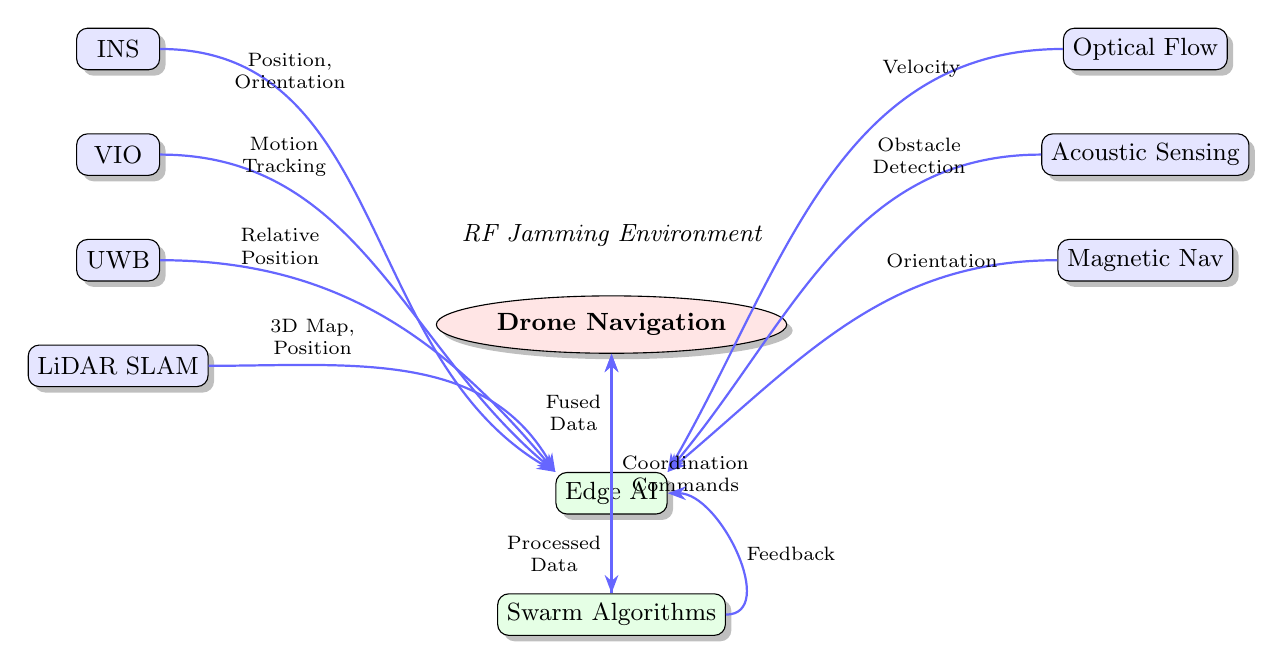
\begin{tikzpicture}[
        box/.style={rectangle, draw, rounded corners, minimum height=1.5em, minimum width=3em, text centered, font=\small, fill=blue!10, drop shadow},
        central/.style={ellipse, draw, minimum height=2em, minimum width=6em, text centered, font=\small\bfseries, fill=red!10, drop shadow},
        arrow/.style={-Stealth, thick, draw=blue!60},
        process/.style={rectangle, draw, rounded corners, minimum height=1.5em, minimum width=4em, text centered, font=\small, fill=green!10, drop shadow},
        node distance=1.5cm and 2.5cm
    ]
    
    % Central drone node
    \node[central] (drone) {Drone Navigation};
    
    % Sensor nodes (left side)
    \node[box, left=3.5cm of drone, yshift=3.5cm] (ins) {INS};
    \node[box, below=0.8cm of ins] (vio) {VIO};
    \node[box, below=0.8cm of vio] (uwb) {UWB};
    \node[box, below=0.8cm of uwb] (lidar) {LiDAR SLAM};
    
    % Sensor nodes (right side)
    \node[box, right=3.5cm of drone, yshift=3.5cm] (optical) {Optical Flow};
    \node[box, below=0.8cm of optical] (acoustic) {Acoustic Sensing};
    \node[box, below=0.8cm of acoustic] (magnetic) {Magnetic Nav};
    
    % Processing nodes
    \node[process, below=1.5cm of drone] (ai) {Edge AI};
    \node[process, below=1cm of ai] (swarm) {Swarm Algorithms};
    
    % Arrows from sensors to Edge AI (curved for clarity)
    \draw[arrow] (ins.east) to[out=0,in=150] node[near start, above, font=\scriptsize, align=center] {Position,\\Orientation} (ai.north west);
    \draw[arrow] (vio.east) to[out=0,in=140] node[near start, above, font=\scriptsize, align=center] {Motion\\Tracking} (ai.north west);
    \draw[arrow] (uwb.east) to[out=0,in=130] node[near start, above, font=\scriptsize, align=center] {Relative\\Position} (ai.north west);
    \draw[arrow] (lidar.east) to[out=0,in=120] node[near start, above, font=\scriptsize, align=center] {3D Map,\\Position} (ai.north west);
    \draw[arrow] (optical.west) to[out=180,in=60] node[near start, above, font=\scriptsize, align=center] {Velocity} (ai.north east);
    \draw[arrow] (acoustic.west) to[out=180,in=50] node[near start, above, font=\scriptsize, align=center] {Obstacle\\Detection} (ai.north east);
    \draw[arrow] (magnetic.west) to[out=180,in=40] node[near start, above, font=\scriptsize, align=center] {Orientation} (ai.north east);
    
    % Arrows from Edge AI to Drone and Swarm Algorithms
    \draw[arrow] (ai.north) -- node[midway, left, font=\scriptsize, align=center] {Fused\\Data} (drone.south);
    \draw[arrow] (ai.south) -- node[midway, left, font=\scriptsize, align=center] {Processed\\Data} (swarm.north);
    \draw[arrow] (swarm.north) -- node[midway, right, font=\scriptsize, align=center] {Coordination\\Commands} (drone.south);
    
    % Feedback loop (cleaner path)
    \draw[arrow] (swarm.east) to[out=0,in=0] node[midway, right, font=\scriptsize] {Feedback} (ai.east);
    
    % Environment label
    \node[above=0.5cm of drone, font=\small\itshape] {RF Jamming Environment};
    
    \end{tikzpicture}
    \caption{Action diagram showing the integration of navigation technologies in a swarm drone UAV. Sensors provide raw data to Edge AI for fusion, with Swarm Algorithms enabling coordination. Fixed arrows ensure clear data flow representation.}
    \label{fig:action_diagram}
\end{figure}

\section{Заключение}

Объединённая система роевых дронов представляет собой комплексное решение, включающее как интеграцию с существующими военными системами НАТО и ВСУ, так и передовые технологии навигации в условиях радиоэлектронного подавления. Трёхуровневая иерархическая архитектура обеспечивает надёжность и масштабируемость, а множественные технологии навигации гарантируют автономность и эффективность работы в сложных боевых условиях.

Ключевые преимущества системы:
\begin{itemize}
    \item Устойчивость к радиоэлектронному подавлению через использование альтернативных методов связи и навигации
    \item Совместимость с существующими системами командования и управления
    \item Автономность принятия решений на уровне роя
    \item Масштабируемость от малых тактических групп до крупных операций
\end{itemize}

Документ готов к компиляции и дальнейшему расширению функциональности системы.

\end{document}